\documentclass[12pt]{article}

% Language setting
% Replace `english' with e.g. `spanish' to change the document language
\usepackage[english]{babel}

% Set page size and margins
% Replace `letterpaper' with `a4paper' for UK/EU standard size
\usepackage[letterpaper,top=2cm,bottom=2cm,left=3cm,right=3cm,marginparwidth=1.75cm]{geometry}



%==========================================================%
% Useful packages
\usepackage{amsmath}
\usepackage{graphicx}
\usepackage{parskip}
\usepackage{csquotes}
\usepackage[colorlinks=true, allcolors=blue]{hyperref}
\hypersetup{
    colorlinks=true,
    linkcolor=black,
    filecolor=magenta,
    urlcolor=cyan,
}
\usepackage{tikz}
\usepackage{import}
\usepackage{colortbl}
\usepackage{ragged2e}
\usepackage{blindtext}
\usepackage{tcolorbox}
\usepackage{graphicx}
\usepackage{xcolor}
\usepackage{listings}


%==========================================================%
% Custom Commands

\newcounter{nbFigures}
\setcounter{nbFigures}{1}
 \newcommand{\myfigure}[3][0.8]{
\begin{center}
    \includegraphics[width = #1\linewidth]{#2}\newline
    \emph{Figure \arabic{nbFigures}: #3}
    \stepcounter{nbFigures}
\end{center}
}
% USAGE
% \myfigure[optional image size 0.1..1]{image path}{title}

\newcommand{\jump}[1][1]{\vspace{#1\baselineskip}}
% USAGE
% \jump[optional number of lines to jump, default = 1]

% \newcommand{\mycomment}[1]{
% \jump
% \begin{tabular}{|p{\linewidth}|}
% \hline
%     \textit{#1} \\
% \hline
% \end{tabular}}
% USAGE
% \mycomment{texte du commentaire}






%==========================================================%
% first page
\begin{document}
ENGINE INFORMATION \hspace{7cm} STARFLEET ONE

\noindent\makebox[\linewidth]{\rule{\paperwidth}{1pt}}
\noindent\makebox[\linewidth]{\rule{\paperwidth}{1pt}}

\begin{center}
    \noindent \textsc{Fluid Injection Starship Engine}

    \noindent \textsc{OD-12 Series}
\end{center}

\noindent\makebox[\linewidth]{\rule{\paperwidth}{1pt}}
\noindent\makebox[\linewidth]{\rule{\paperwidth}{1pt}}

\hspace{12.5cm} CSO Compliant

\vspace{4cm}
\begin{center}
    \Large{\textsc{OD-12v4 Fluid Injection Starship Engine}}

    \Huge{\textsc{Configuration Guide}}
\end{center}



%==========================================================%
% Table of content
\newpage
\tableofcontents




%==========================================================%
% True begining of document

\newpage
\section{Introduction}

This document is the user guide for the \emph{OD-12v4 Fluid Injection Starship Engine}. This document is aimed at the starship engine engineer. The \emph{OD-12} engine series is fully integrated in all modern starship AI systems and it is not necessary to manualy configure the engine. However, this guide meant to be used in case of AI malfunction or shutdown.

\vspace{3cm}
\begin{center}
    \color{red}\Huge{\textbf{Warning}}
\end{center}

Do not manualy configure the engine injection curves before fully reading this guide. A badly configured engine can cause irreparable damages to the crew of your starship (see section 4.3).


\newpage
\section{User interface}
\subsection{Power indicator}
\begin{figure}[!htb]
    \center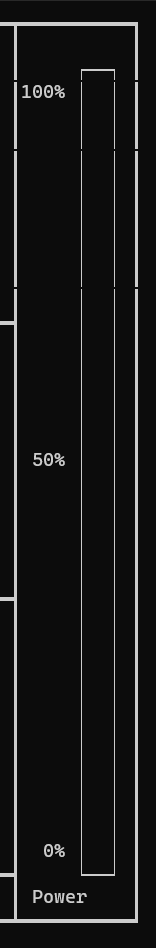
\includegraphics[height=9cm]{images/power_indicator.png}
    \caption{Image of the power indicator pannel}
\end{figure}

This pannel indicates the push force generated by the engine.

\subsection{Starship position pannel}
\begin{figure}[!htb]
    \center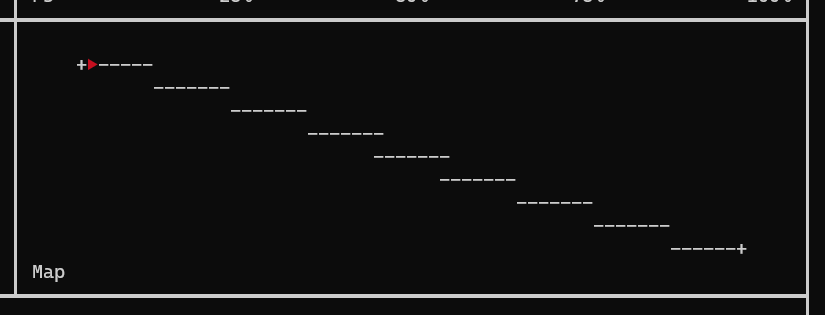
\includegraphics[width=\linewidth]{images/ship_positionment.png}
    \caption{Image of the starship position pannel}
\end{figure}

\newpage
\subsection{Fluid injection curves}
\begin{figure}[!htb]
    \center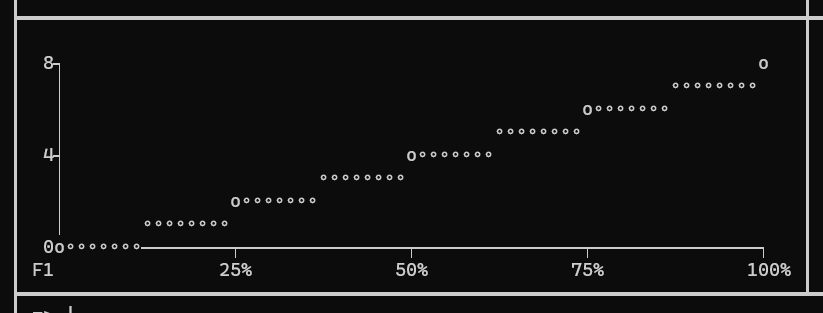
\includegraphics[width=\linewidth]{images/injection_curve.png}
    \caption{Image of the F1 fluid injection curve pannel}
\end{figure}

This graph show on the abscissa the power of the engine, and on the ordinate the injection value for the fluid F1.
In the engine configuration interface, injection curves are available for fluids F1, F2 and F3.

It is the easiest way to represent the amount of fluid injected in relation to the current power of the engine.

\subsection{Information pannel}
\begin{figure}[!htb]
    \center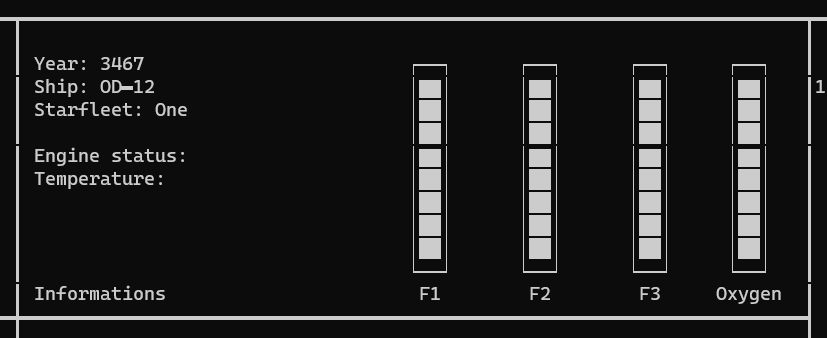
\includegraphics[width=\linewidth]{images/information_pannel.png}
    \caption{Image of the information pannel}
\end{figure}

The information pannel shows the volume of liquid F1, F2 and F3 in the corresponding tanks, as well as the oxygen level of the ship.

\newpage
\subsection{Byproduct monitoring window}
\begin{figure}[!htb]
    \center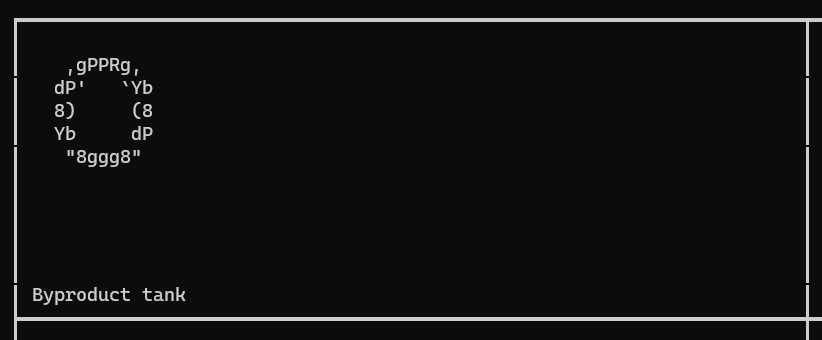
\includegraphics[width=\linewidth]{images/byproduct_tank.png}
    \caption{Image of the byproduct monitoring window}
\end{figure}

This windows helps gauging the amount of byproducts produced by the engine combustion.

\subsection{Input pannel}
\begin{figure}[!htb]
    \center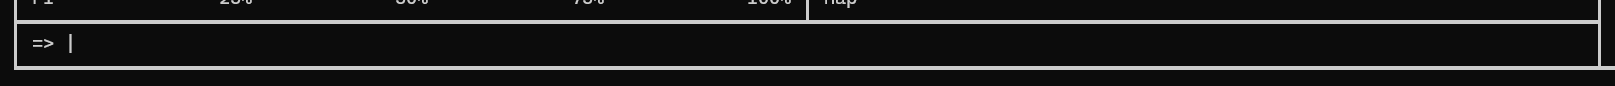
\includegraphics[width=\linewidth]{images/input_pannel.png}
    \caption{Image of the input pannel}
\end{figure}




\newpage
\section{Controls}
\subsection{Interface control}
\begin{tcolorbox}[arc=0mm]
    \textbf{quit}
    \textbf{exit}
    \textbf{q}
\end{tcolorbox}
Exits the engine configuration interface.

\subsection{Engine control}
\begin{tcolorbox}[arc=0mm]
    \textbf{start}
\end{tcolorbox}
Start the engine burning sequence.

\begin{tcolorbox}[arc=0mm]
    \textbf{stop}
\end{tcolorbox}
Stop the engine burning sequence.

\subsection{Set one curve value}
\begin{tcolorbox}[arc=0mm]
    \textbf{[fluid] [power] [injection rate]\newline
    [f1, f2, f4] [0, 25, 50, 75, 100] [0, 1, 2, 3, 4, 5, 6, 7, 8]}
\end{tcolorbox}
Set the given injection rate at given power value for the given fluid.\newline
Example: \emph{f1 50 2} This sets the 50\% injection value of fluid 1 at 2.

\subsection{Set full curve}
\begin{tcolorbox}[arc=0mm]
    \textbf{[fluid] [option] [list of 5 injection values]\newline
    [f1, f2, f4] [full, f] [0, 1, 2, 3, 4, 5, 6, 7, 8]}
\end{tcolorbox}
Set the given curve for the given fluid.\newline
Example: \emph{f2 full 1 2 5 7 8} This sets the injection curve for f2, 0\% has value 1, 25\% has value 2, \dots


\newpage
\section{Engine Combustion}
\subsection{F1 F2 reaction}
The F1 and F2 reaction generates fluid F4 and power following the following curves:

\begin{figure}[!htb]
    \center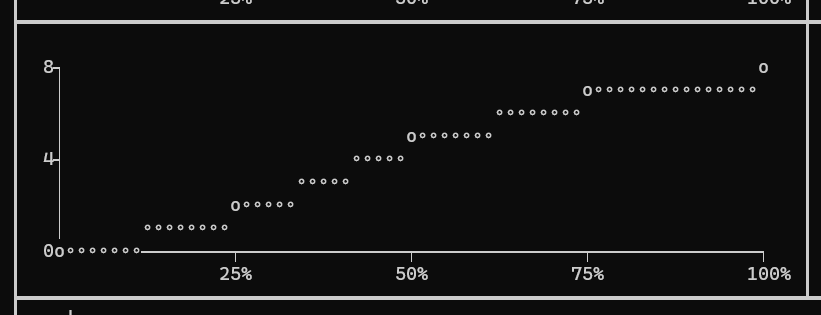
\includegraphics[width=\linewidth]{images/f1f2_f4.png}
    \caption{Graph showing the output of F4 fluid in relation to power for the F1 F2 reaction}
\end{figure}

\begin{figure}[!htb]
    \center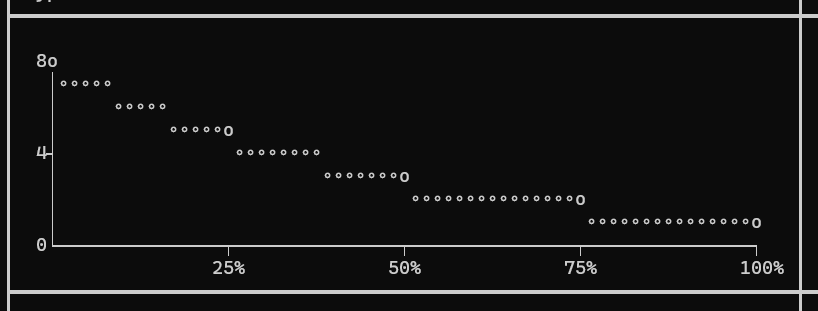
\includegraphics[width=\linewidth]{images/f1f2_power.png}
    \caption{Graph showing the output of power in relation to current power for the F1 F2 reaction}
\end{figure}

\newpage
\subsection{F3 F4 reaction}
The F3 F4 reaction is the main generation of power of the engine. However, it should be closely monitored to ensure that all F4 fluids are consumed by the reaction as F4 is dangerous (see section 4.3)

\begin{figure}[!htb]
    \center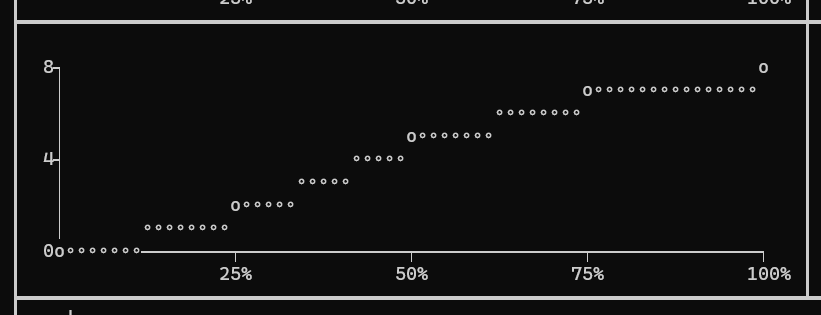
\includegraphics[width=\linewidth]{images/f1f2_f4.png}
    \caption{Graph showing the output of byproducts in relation to power for the F3 F4 reaction}
\end{figure}

\begin{figure}[!htb]
    \center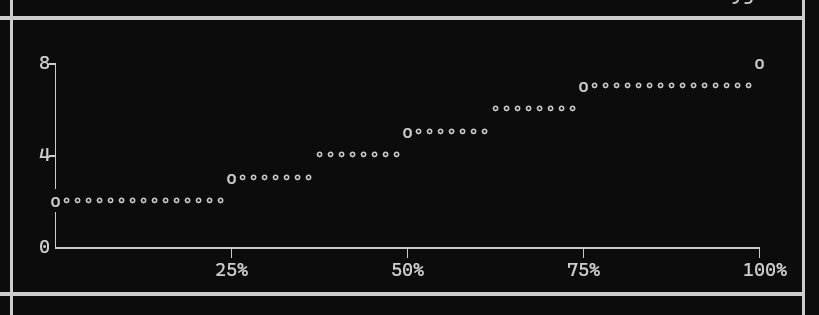
\includegraphics[width=\linewidth]{images/f3f4_power.png}
    \caption{Graph showing the output of power in relation to current power for the F3 F4 reaction}
\end{figure}

\newpage
\subsection{F4 Oxygen reaction}
Every cycles of the engine, remaining F4 fluids in the engine chamber need to be neutralised. This is due to the CSO compliance of the engine. Neutralising F4 fluid consumes the ship's oxygen. The F4 fluide produced by the F1 F2 reaction needs to be fully used in the F3 F4 reaction to avoid ship oxygen depletion.


\subsection{Combustion byproducts}
To ensure compliance with the CSO standards, engine combustion dangerous byproducts are not released into space but stored for later disposal. Treatment of the byproducts ensure it's safety to the crew that will manage the storage of the by products.
No configuration is needed for the byproduct storage.


\subsection{Heat management}
If your engine temperature reaches 200, it will stall. The greatest contributor to the heating of the engine is the creation of by product by remaining F3 fluid in the engine chamber. When the engine is stalled it can be restarted once it has cooled down. Temperature can be lowered by having excess F2 fluid in the engine chamber.


\newpage
\section{Emergency breaking}

The space station auto docking sequence only engages if your speed is lower than 50.
Performing an emergency slow downd can be done if you fear that you will miss your targets. This can be determined by closely inspecting the starship positionment pannel (see section 2.2).

Performing an emergency slow down of the ship is done by flowding the engine with F3 fluid. To ensure maximum efficiency, be sure to cut of injection of fluid F1 and F2 during the breaking sequence.





\newpage
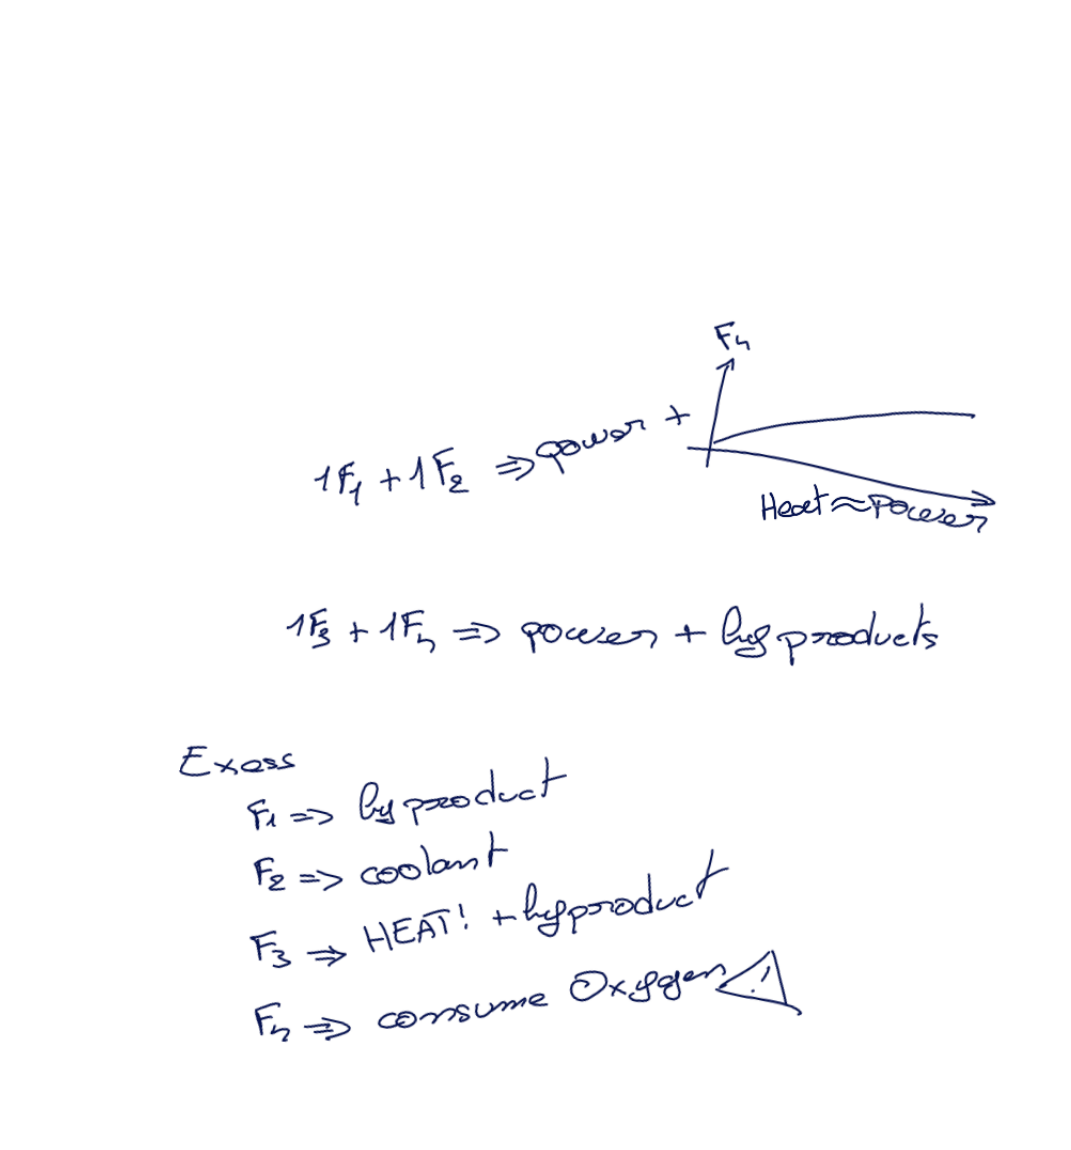
\includegraphics[width=\linewidth]{images/notes.png}









\end{document}
